\documentclass[licencjacka,en]{pracamgr}
% \documentclass{article}

\usepackage{hyperref}
\usepackage{multirow}
% \setlength{\parindent}{0em} % no paragraph indent
% \setlength{\parskip}{1em} % blank space between paragraphs

\usepackage[english]{babel}
\usepackage[utf8]{inputenc}

\usepackage[font=small,labelfont=bf]{caption}
\usepackage{amsfonts}
\usepackage{fancyhdr}
\usepackage{tikz}
\usepackage{amsmath}
\usepackage{amssymb}
\usepackage{float}
\usepackage{graphicx}
\usepackage{hyperref}
\usepackage{subcaption}

\usepackage[numbers]{natbib}
\bibliographystyle{unsrtnat}

\graphicspath{ {./pictures/} }

\autor{Tomasz Garbus}{370795}
\autori{Dominik Klemba}{372710}
\autorii{Jan Ludziejewski}{371158}
\autoriii{Łukasz Raszkiewicz}{371594}

\title{Novelty face authentication with liveness detection using depth and IR camera}
\titlepl{Nowatorskie uwierzytelnianie twarzą z wykrywaniem życia przy użyciu kamery głębi oraz podczerwieni}

\kierunek{Computer Science}

\opiekun{mgr Grzegorz Grudziński%\\
  % Instytut Blabalii Fetorycznej\\
}

\date{June 2018}

\dziedzina{[11.3] Informatics, Computer Science}

%Klasyfikacja tematyczna wedlug AMS (matematyka) lub ACM (informatyka)
% \klasyfikacja{D. Software\\
%   D.127. Blabalgorithms\\
%   D.127.6. Numerical blabalysis}
\klasyfikacja{
Security and privacy\\
\null\hspace{10mm}Security services\\
\null\hspace{20mm}Authentication\\
\null\hspace{30mm}Biometrics
}

\keywords{face recognition, liveness detection, skin detection, depth camera,
biometric authentication, machine learning, neural network, authentication}
% rozpoznawanie twarzy, wykrywanie życia, wykrywanie skóry, kamera głębi, uwierzytelnianie biometryczne, uczenie maszynowe, sieć neuronowa, uwierzytelnianie

\begin{document}
    \maketitle

    \section*{Abstract}

In progress.
Please don't work on that file now.

    \section*{Acknowledgment}
We would like to thank Samsung R\&D Institute Poland for sponsoring this work.
The views expressed in this paper are those of the authors and do not reflect
the official policy or position of Samsung R\&D Institute Poland.

\bigskip \noindent
Furthermore, we would like to thank:
\begin{itemize}
    \item our dissertation advisor,  mgr Grzegorz Grudziński of Faculty of Mathematics,
          Informatics, and Mechanics at University of Warsaw, for supervising our work;
    \item Antoni Jakubiak of Samsung R\&D Institute Poland for overseeing this project;
    \item Karol Brunejko of University of Warsaw's Legal Clinic for legal consultation;
    \item everyone who has contributed to the face dataset;
    \item and everyone who has helped with the creation of this thesis in any other way.
\end{itemize}


    \tableofcontents

    \chapter{Introduction}
    In the world of authentication, there is always a trade-off between
    convenience and security. We would like to compare commonly used authentication
    methods with regard to both factors and argue that face recognition is more than
    a good balance between the two -- it does very well in terms of both security
    and convenience.

    \section{Conventional authorization methods}
        \subsection*{Passwords}
            Passwords come in various forms and cannot be easily placed on a
            security-convenience curve. Their strength is exponentially dependant
            on their length.

            The strength and form of a password often depend on the context of its
            use. For instance, passwords used for unlocking the screen in a mobile
            device tend to be simple and quick to input -- a pattern to draw, a
            $4$ to $8$-digit pin, in rare cases -- an alphanumeric sequence.
            Passwords used for bank accounts, on the other hand, can be undeniably
            strong, to the point of being a randomly generated sequence of lower
            and upper letters, digits and special characters.

            With those two extreme examples in mind, we can conclude that passwords
            can be very secure and they can be very convenient. But that does not
            imply that passwords can be very secure and very convenient at the
            same time.

            Another thing to keep in mind is that passwords are an authentication
            method that relies on user's \textit{knowledge} -- knowledge of the
            secret code and the ability to remember it at all times.

            That, however, is changing. Password managers and credential managers have been taking
            the responsibility of not only storing the passwords but generating
            them too. The user does not have to know their password -- it is sufficient
            that the password manager knows it and that the user is in \textit{control}
            of password manager. It is a good defense against phishing attacks,
            assuming the user can be tricked into giving their password more
            easily than the password manager.


        \subsection*{Hardware tokens and magnetic cards}
            Sometimes to protect valuable resources,
            something stronger than standard password is needed.
            Hardware tokens such as U2F-like tokens or password-protected RSA SecurID
            and magnetic cards are good choices then.
            Those authorization methods rely on user's
            \textit{possession} of said token or magnetic card. To
            gain access to the victims resources, an attacker must take gain
            possession of the physical key, whether it is a U2F- or SecurID-like token.
            Magnetic cards are more vulnerable to attacks -- it is possible to
            conduct an attack without obtaining the card itself, but instead
            being within its close range.

    \section{Biometric authentication}
        Conventional authorization methods are based on \textit{possession},
        \textit{knowledge} or \textit{control} over some resource. Usually, the
        resources in question are copyable.
        We have no intention of undermining such methods, because they can be
        extremely secure if designed well.

        Instead, we would like to focus on another paradigm of authentication,
        which relies on \textit{being} -- being the right person to authorize.
        With this approach, the authorization keys -- users -- are unique and non-copyable. However,
        their uniqueness is as good as the authorization system's ability to
        distinguish between them.

        Biometric authentication is a set of techniques striving to recognize a
        human being by their appearance, body or behavior.

        \subsection*{Fingerprints}
            % If we want some link to literature, I'd go with Janusz Zajdel's Limes
            % Inferior. It has the exact theme of chopping off fingers as a form
            % of mugging - in the created world each fingerprint had some
            % "foodstamps" assigned. What's interesting about this example,
            % the fingerprints are checked electronically in the book and it
            % was published in 1982. -tomek
            Fingerprints have been used for a long time for identifying their
            owner, especially in criminology. They are perfectly fine in terms of
            distinguishing people as everyone's fingerprint is unique. Moreover,
            even if there happened to be two people with identical fingerprints,
            it would be an extremely unlikely coincidence for one of them to try
            to hack the other.
            Unfortunately, while users are a non-copyable resource, their fingerprints
            are indeed copyable.

        \subsection*{Behavioral biometrics}
            Behavioral biometrics have been making their way into
            the banking industry. They are a set of techniques supporting the
            conventional authentication, by learning, and verifying, user's
            preferences and habits, such as (by \citeauthor{behavioral}):
            \begin{itemize}
                \item Behavioral qualities of the input data, such as typing
                      speed or touchscreen interactions and their timing;
                \item Supporting contextual factors of the current transaction,
                      such as user device type, IP address, geolocation; and
                \item The user’s historical behavioral factors, such as the
                      typical timing of user access, prior purchasing or access
                      patterns, etc.
            \end{itemize}
            The downside is, behavioral biometrics are not a standalone solution.
            They are more of an anomaly detection system reinforcing the authentication
            system.

        \subsection*{Face recognition}
            Face recognition is an authentication method that is both convenient
            and secure -- in theory. It has been used in smartphones, tablets
            and laptops for several years now, mostly to unlock the device, but
            never really trusted enough for securing more vulnerable resources.
            Faces, like fingerprints, are unique, but their uniqueness cannot be
            taken for granted. For instance, a static, two-dimensional picture of
            a face is perfectly copyable.

    \section{Liveness detection}
        To design a secure face recognition based authentication system,
        one should ensure the user's face is non-copyable. Only then will the
        system fully comply to our paradigm of relying on \textit{being} instead
        of \textit{possession}.

        This can be achieved by adding liveness detection to the authentication
        process. Liveness detection itself can be based on multiple techniques.

        \subsection*{Existing methods}
            Various mobile phone manufacturers have implemented methods attempting to
            detect whether the visible face is actually a human and not a photo.
            For example, users were asked to blink or smile to unlock their phones.

            Such methods definitely increase the security of face recognition,
            but they are inconvenient to the user -- ideally, one would not need to take
            any action to unlock their device -- and were often easily hacked by having
            additional photos of the owner, even fake ones with the eyes being covered.

        \subsection*{Depth channel}
            Using a depth channel in addition to a flat image is a form of liveness
            detection itself.
            When implemented well, such system should block all attempts to authenticate
            using a photo of an authorized person.
            However, it could still be broken using a detailed mask of that face.
            While that would require a lot of effort, it is a realistic way to break
            into for example a stolen phone of an important person.

        \subsection*{Pulse detection}
            Determining a person's pulse from a video is not a new idea.
            We have found existing implementations of programs that detected the user's
            pulse, using for example a webcam \cite{pulsedetector}.
            Unfortunately, we found out that such liveness detection method would be
            too slow for common authentication purposes.
            Detecting the pulse takes several seconds and requires the face to remain
            in one particular spot through the entire procedure.
            Therefore we we abandoned further research on this subject.

        \subsection*{Skin recognition}
            The liveness detection idea which we decided to research is skin recognition.
            With a reliable method to detect whether real skin is visible in the camera,
            it should be nearly impossible to authenticate without actually showing
            the owner's face to the camera.
            Our proposed skin recognition ideas will be described later in this paper.

    \section{Results}
        In our work, we have focused on skin recognition and face authentication
        with depth channel.

        \subsection*{Skin recognition}
            We have developed several skin recognition techniques working with different
            sets of light wavelengths. We have also constructed a simple hardware prototype
            and experimented with machine learning approaches to per-pixel skin recognition.

        \subsection*{Face authentication}
            We have constructed a depth + infrared face dataset and evaluated different
            machine learning approaches to face recognition. We have measured the
            effect of authentication time limit on its effectiveness and the trade-off
            between security and convenience.

    \section{Skin recognition}
    Motivations of liveness detection are described above.
    Idea to use light reflectiveness comes from fact that
    every material has own, unique spectrum. [TODO: LINK NEEDED]
    We have been focused on infrared light mostly by papers about
    skin detection in smart cars. [TODO: LINK NEEDED]

    With skin recognition system, it would possible to
    detect face much faster that with ML approach,
    as (at least ours) all ideas how to use IR
    to decet human sin are besed only on one pixel,
    so it's easy to parallelize.
    A lot of out attempts are very simple in sense of math,
    so it's also very fast -- just few multiplications and sumations.

    \subsection{How it works?}
        WIP

    \subsection{Technical aspect -- how camera works?}
        To think about security aspect of skin detection,
        it's critical to understand how image sensors works.
        Most common are \textit{CCD} (\textit{charge-coupled device})
        and \textit{CMOS} (\textit{complementary metal-oxide-semiconductor})
        [TODO: LINK NEEDED]. % Most common?
        Due to better quality, as well as sensitiveness, for security reasons
        it probably would be better to use CCD.
        However, both matrices have same problem -- limitation on wavelength sensitivity.
        Such sensors are sensitive to wavelengths aproximetly up to 1050nm,
        which may be serious limitation as skin ligthen with greater wavelength has
        more undifferentiated characteristics.
        Therefore looking for best possible skin detection method,
        it may be convenient to assume that other type of light sensitive matrices
        are in reach of inventor.
        Nevertheless we were limited to very common cameras.

        TODO: Paragraph about light sensors materials and other types of image sensors.
        Paragraph under maintenance. May dissapear.

        We are describeing one possible realization, keep in mind that
        there are more solutions than that, but we don't find them usfeful in our problem.

        \subsubsection*{Monochrome}
            As image sensor is matrix build from many small photodiodes,
            % TODO: in fact working like...
            it's natural to create monochromatic image.
            Because photodiodes don't distinguish different
            wavelength, only light intensity, it's hard
            to measure light reflectiveness.
            The only possible way to do that is to
            make different picture for every wavelength.
            It's not easy, as you have to
            provide your own lighting and somehow remove
            light coming from other sources.
            Also, all pictures have to be made in
            a~very short time interval, as the subject
            cannot move between shots.

        \subsubsection*{Multispectral imaging}
            Multispectral imaging is answer to
            problem of object's move,
            way to measure every wavelength intensity in one picture.
            Probably easies way to describe it is to look at RGB camera.
            There every photodiode is responsible for exacly one colour,
            where as colour we understand wavelength interval (it's important
            to understand, that we can consider any wavelength interval as one colour).
            And result picture is built from small squares (mostly $2 \times 2$)
            of photodiode matrix data.
            There may be more than just  three colours in fact.
            For example, you may find camera which see two types of ''green''.
            Mostly, at the end everything is converted to known RGB format.

            \begin{figure}[H]
                \caption{RGB image sensor matrix with two types of green -- sensors assignation.}
                \centering
                \includegraphics{RGB-matrix}
                \label{fig:RGB-matrix}
            \end{figure}

            Software receives from camera imformation with light intensity at every
            sensor and information which colour it sees.

            One from possible realisations of reducing the range
            of light visible through the sensor is to take standard image sensor which
            may see full specturm of light ($350$-$1050$nm.) and
            place filters in way that only specific light will reach choosen photodiode.

            \begin{figure}[H]
                \caption{Visualisation of how filters works.}
                \centering
                \includegraphics[scale=0.40]{RGB-filter}
                \label{fig:RGB-filter}
            \end{figure}

        \subsubsection*{Hyperspectral imaging}
            Hyperspectral imaging is creating pictures using camera with
            capabilityy to distinguish many and many of colours (more like hundreds or thousands)
            instead of just few.
            It would be very helpful, obviously, in skin-detection device,
            but there is very little chance to see such device in mobile phones soon.

    \subsection{Technical aspect -- how it may be created?}
        As we know how camera works, we can say that there are only two ways of
        building skin detection mobile device.
        \subsubsection*{Monochrome}
            We can work without filters (or with one for whole camera),
            but then we have to make picture for every wave lenght.
            Also, we need one diode with that very wavelength we want.
            It's easier method to build in phone, but taking pictures
            must be very fast.

            Bigest pros of that solution is possibility of lighting
            with different LEDs in random moment of time, so hackers
            will no be able to play with own diods to modify result.

        \subsubsection*{Multispectral imaging}
            Also there is possibility to use filters with specific infrared colours.
            But important here is avoiding standard smoothing algorithms used
            in cameras. We truly need real light intensity from every sensor.
            Not smoothed or reduced one.

    \subsection{Our attempts}

        \subsubsection{Detecting reflectiveness using Kinect}
            Our first idea was to use a Kinect v2 depth and infrared camera to detect
            how well does a surface reflect light.
            Kinect v2 cameras have their own source of infrared light and they make
            a very good job at filtering other sources of light.
            So, for each pixel on the infrared image, we know how much light coming
            from the Kinect's light emitter was reflected in that particular place.
            Also, Kinects are depth cameras, which additionally gives us the information
            on how far away from the camera is the object visible on that pixel.

            Since the source of light is in the same device as the camera, the distance
            seen on the depth image is also the distance from the light emitter.
            This is an important observation, because we know how distance affects how
            much light arrives at a particular place. % might need a better wording
            If we have a source of light that, at a given distance, lights up a
            1cm $\times$ 1cm square of a flat surface with a particular amount
            of light, then at double that distance it will light up a 2cm $\times$ 2cm
            square with the same amount of light, which means that the same amount
            of light is distributed over a 4 times larger surface, so the
            intensity of light has to be 4 times lower than before.

            With those observations, we took pairs of IR and depth images, and for each
            pixel calculated a new value of $ir-intensity \cdot depth \cdot depth$,
            which should estimate how well light was reflected at that point,
            regardless of distance from the camera.

            \begin{figure}[H]
                \caption{An unprocessed IR photo, and an image calculated using
                the method described above.}
                \centering
                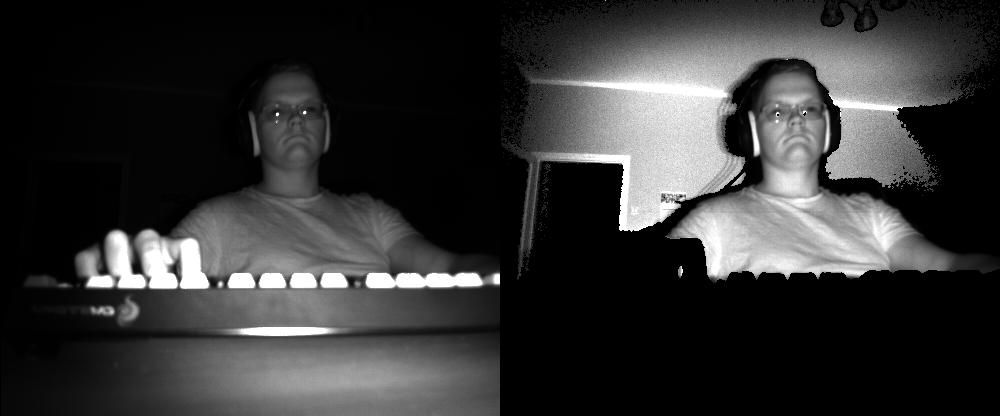
\includegraphics[width=\textwidth]{skin_kinect_1}
                \label{fig:skin_kinect_1}
            \end{figure}

            As seen on figure \ref{fig:skin_kinect_1}, we have accidentally created
            a night vision camera (please note that some of the black areas are there because Kinect cameras do not give depth data for objects closer than 50cm)
            -- but this means that our idea is to some extent working, because the point
            of it was to make objects in the distance indistinguishable from those close
            to the camera.

            However, one this that is not considered in that method is that objects
            can also be at different angles to the camera.
            A sheet of paper perpendicular to the source of light will reflect more
            light to the Kinect than it would reflect if it was at a 45 degrees angle.

            \begin{figure}[H]
                \caption{Three IR images processed with the described method, with a
                manually determined interval of values marked red.}
                \centering
                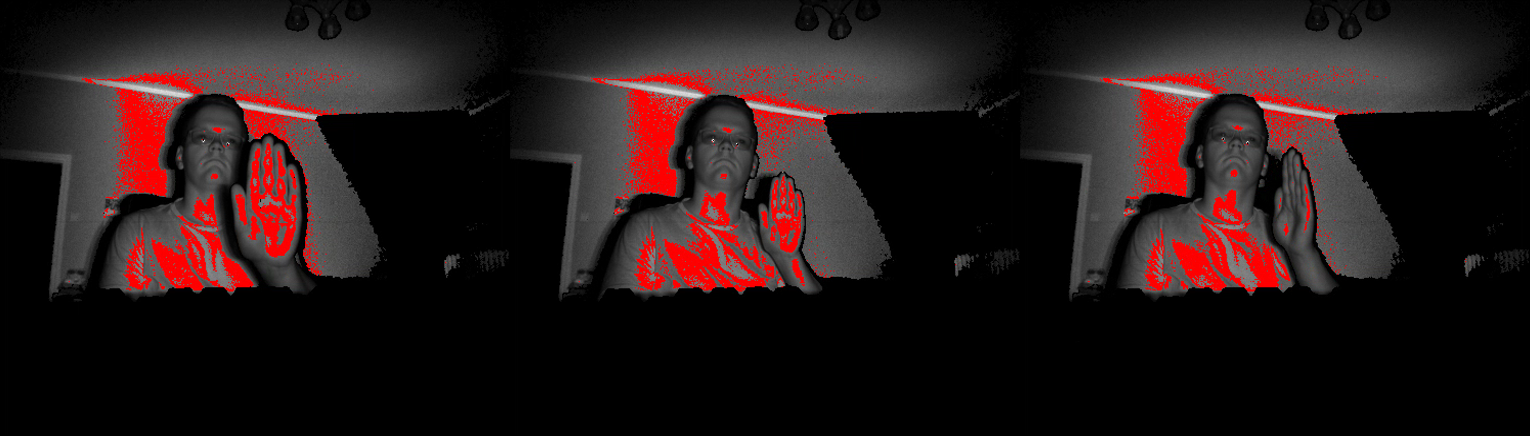
\includegraphics[width=\textwidth]{skin_kinect_2}
                \label{fig:skin_kinect_2}
            \end{figure}

            We have manually selected an interval of values and marked them red, which
            can be seen on figure \ref{fig:skin_kinect_2}.
            On the first two pictures there, the hand is at the same angle, but at a
            different distance to the camera.
            It is visible that the calculated values remained very close regardless
            of the distance, which was a success.
            However, on the third picture, the hand is at a different angle and
            that changes how it reflects light towards the camera, which makes the values
            different.

            Knowing the depth value and certain properties of the camera, it is possible
            to calculate the 3D coordinates of each pixel.
            With that information, it is possible to calculate the angle towards the
            camera between each two pixels, and then use that value in the method above
            to make it independent of angles.
            However, our attempts to do this were unsuccessful, possibly because the
            depth camera is not precise enough.
            % TODO Dominik: maybe describe briefly the mathematical details of what
            %               was attempted

        \subsubsection{Using three infrared wavelengths}
            \subsubsection*{Prototype}
            With the previous method using only one light wavelength (the one emitted by
            Kinect), we decided to take photos using three different wavelengths.
            This gives the opportunity to analyze how does the way the objects reflect
            light changes with regard to light wavelength, instead of directly looking
            at how bright a point is.

            To make any research, we had to take three photos of the same object
            reflecting three different wavelengths of infrared light.
            The camera, the infrared light sources, and the photographed object
            had to be in the same position for all of the photos.
            An ideal way to do this would be to use a spectral camera, but they are
            very expensive and we were not able to use one.

            One possible way to take a photo of how a certain wavelength is reflected
            would be to use a filter that only lets that wavelength to pass through it.
            However, changing filters on the camera between taking photos would take
            a lot of time, which would create a risk of changing the relative position
            of the object and the camera, which is unacceptable.

            We borrowed a mobile phone which had a filter mounted on its front camera
            that allowed various wavelengths of infrared light, but not visible light.
            This opened up the opportunity to take a different approach -- instead
            of filtering the selected wavelength, we want to illuminate the object
            using only that wavelength.

            We purchased diodes emitting light in the following wavelengths:
            850nm, 890nm, 940nm. Those diodes were connected to an Arduino board.
            We used two diodes of each wavelength, and mixed their positions to
            make sure that the centers of sources of light at each wavelength
            are as close as possible.

            \begin{figure}[H]
                \caption{Arduino board with six IR diodes.}
                \centering
                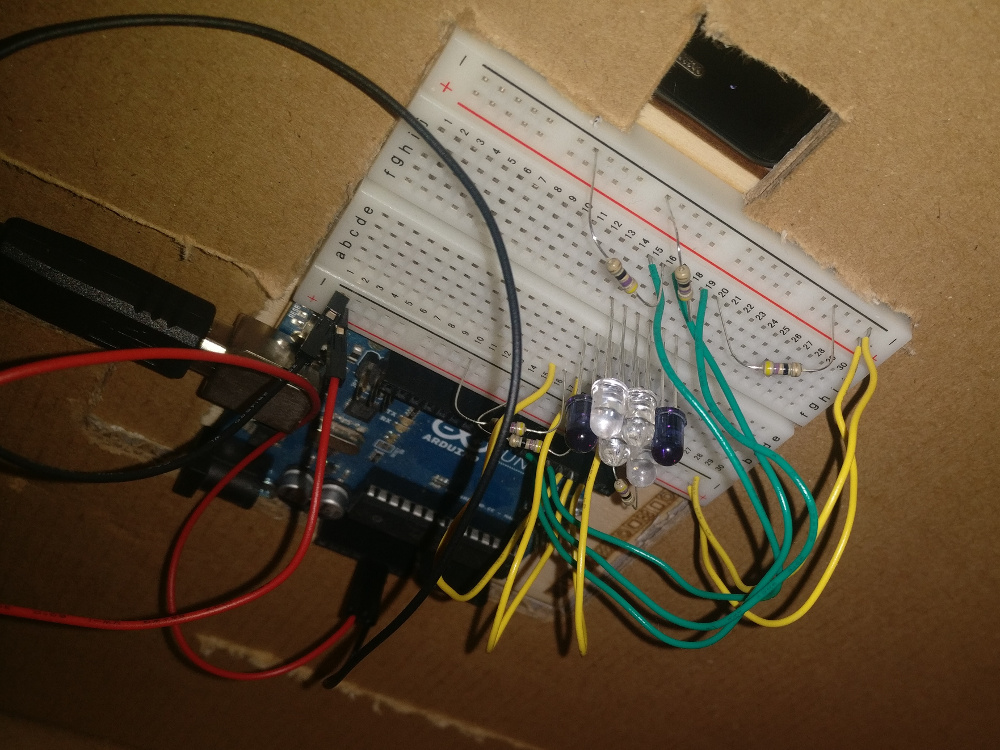
\includegraphics[height=7cm]{arduino_1}
                \label{fig:arduino_1}
            \end{figure}

            Since taking all three photos at the same time would be impossible,
            we stabilized the camera and the diodes by putting them in holes
            in a cardboard box.

            \begin{figure}[H]
                \caption{Outside view of the Arduino board and the camera.}
                \centering
                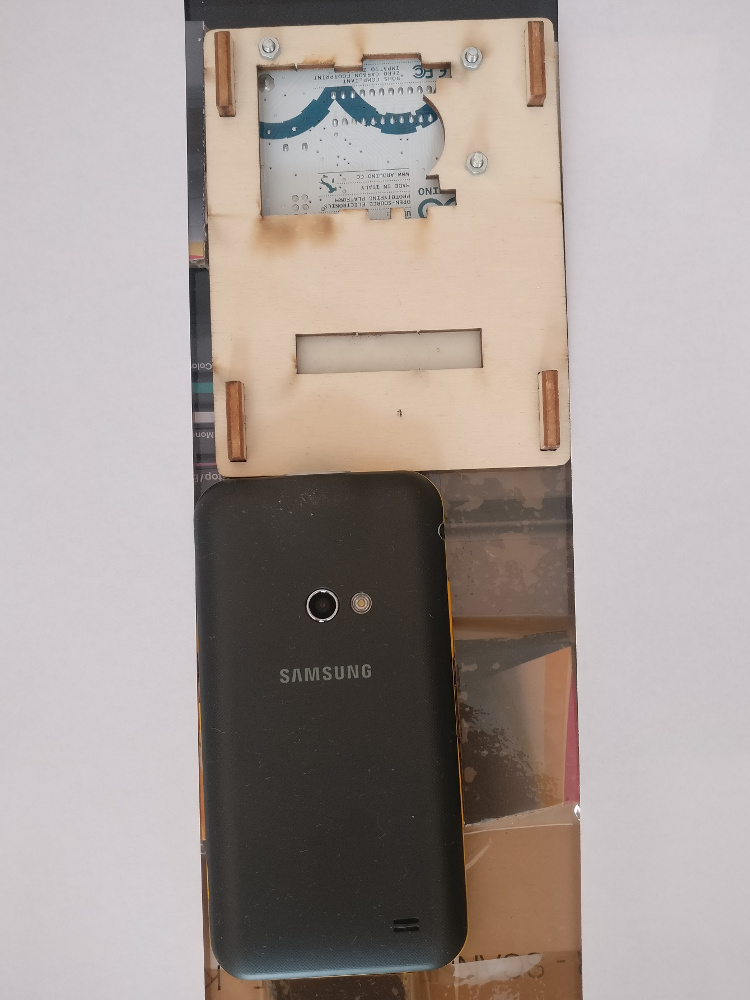
\includegraphics[height=7cm]{arduino_2}
                \label{fig:arduino_2}
            \end{figure}

            With this setup, all that remained to do was to take more photos.
            The camera and the phone were stable, but when photographing for example
            a human hand, it might move.
            The photos have to be taken in the smallest possible intervals
            and human interaction can not be required while taking them,
            because that could result in moving the camera or the diodes.

            Turning specific diodes on and off was a rather easy task.
            Arduino is by definition programmable, so we just wrote a program that
            listened to data sent on a USB cable and turned on the requested diode.\\
            We found an Android app \cite{opencameraremote} designed to take photos
            remotely when commanded so from another phone with a special pilot app.
            It is open source, so we read its source and found out that it just sends
            simple broadcast messages through LAN.

            With this information, we were able to write a Python script that did the
            following:

            \begin{itemize}
                \item connect to Arduino through USB, turn on 850nm diodes
                \item wait 0.75 seconds
                \item send a broadcast message to take a photo
                \item wait 0.75 seconds
                \item turn on 890nm diodes
                \item wait 0.75 seconds
                \item take a photo
                \item ... -- analogical procedure to take a photo with 940nm light
            \end{itemize}

            Since we were using only the front camera from a relatively old phone,
            we had to take a 1.5 seconds break between each photo -- otherwise
            there was a significant chance of the camera app not catching one of the
            broadcasted commands and taking only two photos.
            The time between the first and last of three photos was 3 seconds,
            and that was an acceptable delay to make sure that the photographed
            object was in a stable position.

            \begin{figure}[H]
                \caption{Photos taken with 850nm, 890nm, and 940nm light respectively.}
                \centering
                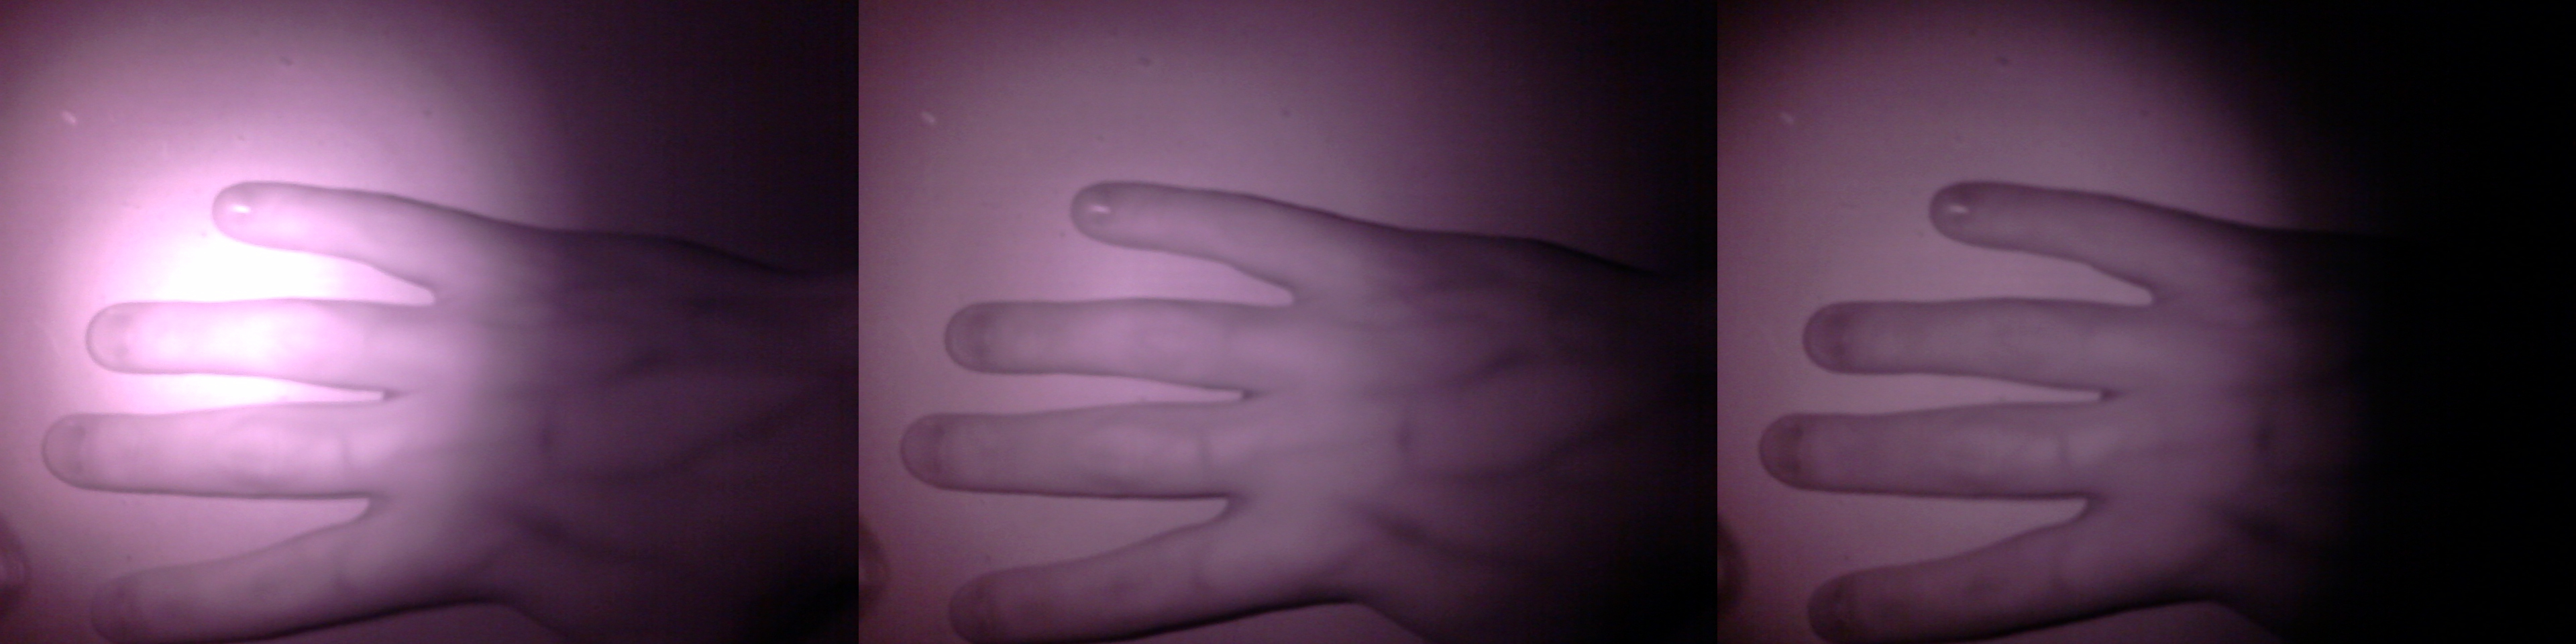
\includegraphics[width=\textwidth]{ir_photos}
                \label{fig:ir_photos}
            \end{figure}

            \subsubsection*{Detecting skin}
            TODO @Dominik: describe the machine learning method used for skin detection

            \begin{figure}[H]
                \caption{TODO}
                \centering
                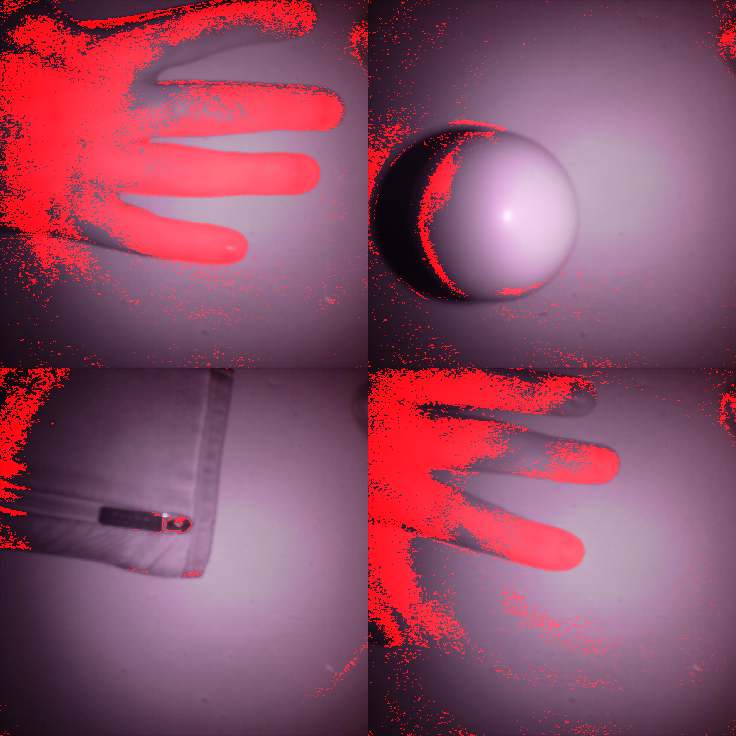
\includegraphics[width=10cm]{skin_results}
                \label{fig:skin_results}
            \end{figure}

    \subsection{Results}
        The results achieved by our skin detection were far from perfect,
        however we still think that using infrared photos to analyze surface
        reflectiveness and using that to detect skin is a promising method.
        We were very limited by the low quality photos, overall lack of
        high quality hardware, and our lack of knowledge in electronics,
        but were still able to achieve results that visually make sense.
        With more resources, we believe this could increase security of
        face authentication solutions.

    \subsection{RGB skin detection symulation}
        Using RGB to deteckt skin on picture.
        Mtoivations.

        Description of not ours solutions.

        \subsubsection*{Case-study}
            Description of problem using math.
            Final algorithm.

    \section{Face authentication}
    Face recognition is a problem that has been around for a while and
    human-level solutions have been developed, such as FaceNet\cite{arXiv:1503.03832}.
    However, there are many subtleties to face recognition in mobile devices
    security, in particular when using unconventional cameras.

    From the security context, false positives are very problematic. This observation alone
    poses two questions:
    \begin{itemize}
      \item How to measure a model's performance to punish false positives?
      \item How to maximize our chosen score measure?
    \end{itemize}
    We have tackled two problems in our research -- multi-class and binary classification.
    Binary classification is more adequate to the possible applications of our research.
    Multi-class classification allows the reader to compare the achieved results
    with other face recognition models.

    The second observation is more optimistic: the front camera of a mobile is capable of
    capturing relatively many frames per second. We decided not to constrain our
    methods to a classification based on a single frame.
    Moreover, a large training set can be built
    when adding a new user to the device -- it is not unreasonable to make that procedure
    longer for increased security. We aimed to take advantage of those factors.

    \subsection{Data set}
    We have set requirements for our dataset, aiming to reflect real-life
    appliances:
    \begin{itemize}
        \item \textbf{depth and IR channels}: in real-life appliance, leveraging
        the infrared camera allows equally good vision regardless of lighting
        conditions.
        \item \textbf{various vertical angles}: when a user is looking at their
        mobile device,
        their head may be placed at various angles along the vertical axis.
        However, it is reasonable to assume that the angle along the horizontal
        axis will be small, especially if the user is consciously trying to
        unlock the device.
        \item \textbf{many frames per subject}: when a new user is being added
        to a mobile device's authentication system, it is acceptable to require
        them to look at the camera, at various angles, for a short period of
        time. Many frames can (and should) be taken.
    \end{itemize}

    There are several good databases for face recognition with depth camera:
    The EURECOM Kinect Face Database\cite{eurecom},
    RGB-D Face database \cite{vapaaudk},
    The Florence Superface dataset\cite{superface}. However, none of them was
    deemed suiting for our project, primarily due to the lack of IR channel.
    Thus, we have decided to build a dedicated dataset.

    \subsubsection*{Data collection}
    The dataset consists of $44$ subjects: $36$ males and
    $8$ females, mostly aged $20$-$25$. Each subject has been asked to
    follow an object with their entire head, making two cycles of slow,
    continuous movements: \texttt{up $\to$ center $\to$ down $\to$ center $\to$
    left $\to$ center $\to$ right $\to$ center}.
    That procedure has resulted in approximately $20$ seconds of footage per
    subject.

    IR and depth frames are synchronized, taken at $10$ FPS rate.

    Dataset contains also RGB frames taken at $10$ FPS rate, not synchronized
    with IR and depth frames.

    The procedure performed to collect photos of a single person took around $20$-$30$ seconds.
    We believe it could be proposed as a part of mobile device's first time security configuration.

    \subsubsection*{Test set}
    For the test set, we have chosen approximately first $25\%$ of
    frames from each subject -- the first two vertical head rotations.

    \subsubsection*{Samples}
    \begin{figure}[H]
    \caption{One of the subjects from the database -- the first $269$ IR frames.}
    \centering
    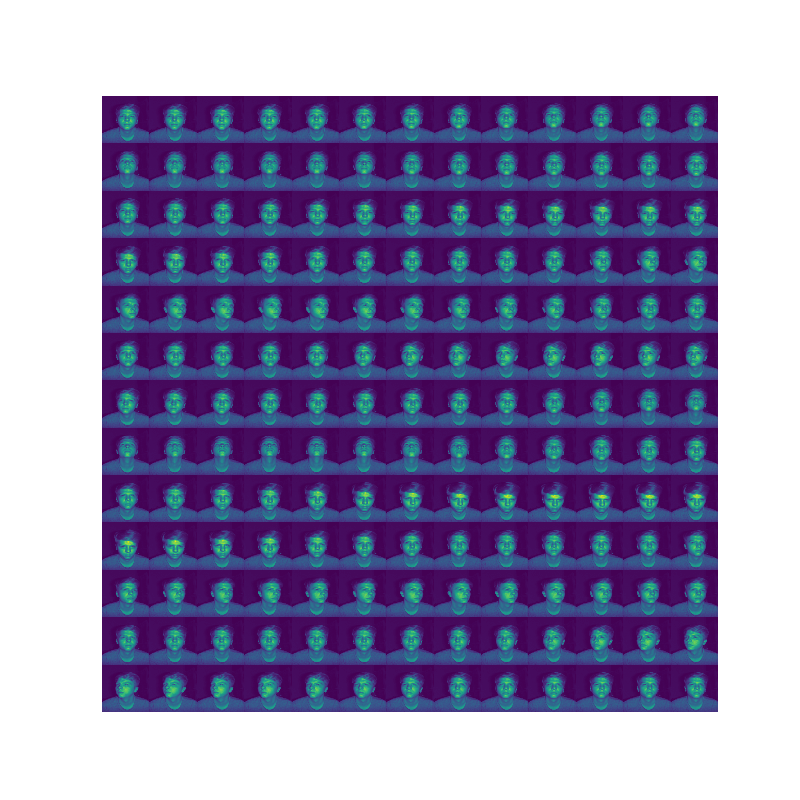
\includegraphics[scale=0.5]{tiled_faces_ludziej}
    \end{figure}

    \subsection{Face angle detection}
    \label{sec:angledetection}
    Using depth camera, we can extract more structural features of an image,
    and normalize the face angle. Face is positioned in a cube, and position vector is computed
    by finding three points located on face, describing the surface
    and computing its orthogonal vector. We define face position
    as the angle between the computed vector and vector $[0,0,1]^T$ pointing towards the camera.
    We have chosen the points as the middle of each eyebrow and the middle of the chin and compute them with
    same library we use for face trimming (as an average between chosen subsets of points). Worth
    mentioning is that choosing points too close to edge of face (as most algorithms do)
    detected on 2-dimensional image, might turn algorithm unstable, because small error can place the point on the background,
    far away in third dimension.


    \begin{figure}[H]
    \caption{Detecting the angle of face. The face orthogonal vector is positioned between eyebrows, face points are marked yellow}
    \centering
    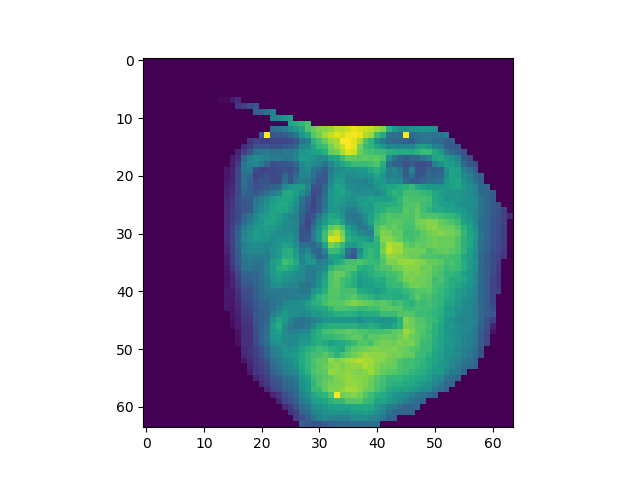
\includegraphics[scale=0.5]{angle}
    \end{figure}


    \subsection{Normalization}
        \subsubsection*{Depth mean and standard deviation normalization}
        Let $F$ be the set of all points belonging to the trimmed face and
        $d(p)$ -- depth of the point $p$. Let $\mu$ denote the mean depth, i.e.
        $\mu = \frac{\sum\limits_{p \in F}{d(p)}}{|F|}$ and $\sigma$ -- standard
        deviation, i.e. $\sigma = \sqrt{\frac{1}{|F|} \sum\limits_{p \in F}{(d(p) - \mu)^2}}$.
        For each pixel $p$, its new depth is calculated as:

        \begin{center}
        $
          d'(p) = \begin{cases}
                  d(p) - \mu &\quad\text{if}\ |d(p) - \mu| \leqslant 2 \cdot \sigma \\
                  0 &\quad\text{otherwise}
                  \end{cases}
        $
        \end{center}


        Lastly, all depth values are scaled to the interval $[0..1]$:
        \begin{center}
        $
          d''(p) = \frac{d'(p) - min(\{d'(r)\ |\ r \in F\})}{max(\{d'(r)\ |\ r \in F\}) - min(\{d'(r)\ |\ r \in F\})}
        $
        \end{center}

        \subsubsection*{Face angle normalization}
        Depth channel provides substantial information about faces' geometry, thus allowing
        a meaningful normalization method -- rotation to the frontal position.

        With our ability to detect face angle (\ref{sec:angledetection}), we can obtain
        three values: $\theta_x, \theta_y, \theta_z$ -- angles along each axis.

        The face can be represented as a cloud of $3$-dimensional, "colorful" points.
        Point $p$ is defined as a vector $[x_p, y_p, z_p, ir_p]^{T}$.

        Let $R_x(\theta_x), R_y(\theta_y), R_z(\theta_z)$ denote the rotation matrices
        for $X, Y, Z$ axes, as follows:
        \[
        R_x(\theta_x) =
        \begin{bmatrix}
        1 & 0 & 0\\
        0 & cos(\theta_x) & -sin(\theta_x)\\
        0 & sin(\theta_x) & cos(\theta_x)
        \end{bmatrix}
        \]
        \[
        R_y(\theta_y) =
        \begin{bmatrix}
        cos(\theta_y) & 0 & sin(\theta_y)\\
        0 & 1 & 0\\
        -sin(\theta_y) & 0 & cos(\theta_y)
        \end{bmatrix}
        \]
        \[
        R_z(\theta_z) =
        \begin{bmatrix}
        cos(\theta_z) & -sin(\theta_z) & 0\\
        sin(\theta_z) & cos(\theta_z) & 0\\
        0 & 0 & 1
        \end{bmatrix}
        \]
        The operation of rotating a single point is a product of its coordinates and the three rotation matrices:
        \begin{center}
        $
        \begin{bmatrix}
          x_p\\
          y_p\\
          z_p\\
          ir_p
        \end{bmatrix}
        \cdot
        \begin{bmatrix}
          R_x & 0_{3}^T\\
          0_{3} & 1
        \end{bmatrix}
        \cdot
        \begin{bmatrix}
          R_y & 0_{3}^T\\
          0_{3} & 1
        \end{bmatrix}
        \cdot
        \begin{bmatrix}
          R_z & 0_{3}^T\\
          0_{3} & 1
        \end{bmatrix}
        $
        \end{center}


        \begin{figure}[H]
        \caption{Face from angle detection subsection, transformed.}
        \centering
        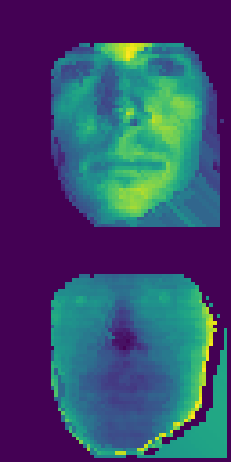
\includegraphics[scale=0.5]{angle_transformed}
        \end{figure}

    \subsection{Preprocessing techniques}
    We have used several different preprocessing techniques.
        \subsubsection*{Trimming faces}
        \label{sec:trimming}
        During the process of collecting the dataset, each subject has been
        recorded in only one set of clothes (the ones they were wearing at the
        time), one hairstyle and the background may slightly vary among the
        subjects (the background behind subjects recorded at $12$ a.m. is
        likely to be brighter than behind the subjects recorded at $4$ p.m.).

        Since a classifier might leverage those factors, photos have been
        trimmed to polygons containing the faces. Such polygons have been
        found with Face Recognition library \cite{facerecog} on IR photos.
        Depth photos have been trimmed accordingly.

        \begin{figure}[H]
        \caption{Before and after trimming the face.}
        \centering
        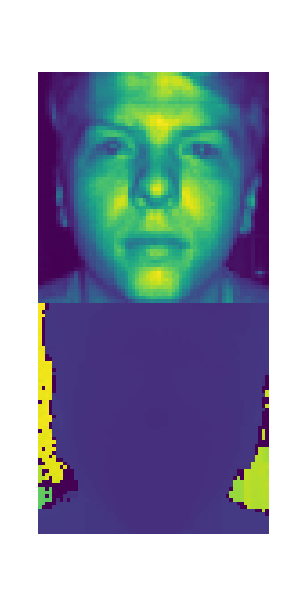
\includegraphics[scale=0.25]{before_trim_ludziej}
        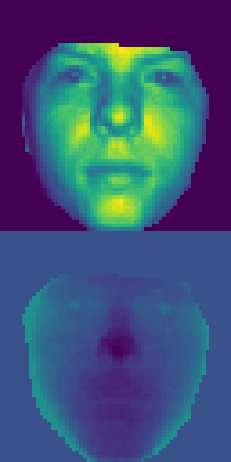
\includegraphics[scale=0.25]{after_trim_ludziej}
        \end{figure}

        \subsubsection*{HOGs}
        To transform 2-dimensional images into 1-dimensional feature descriptors,
        we used standard preprocessing called Histogram of Oriented Gradients, commonly used in
        object detection (\citeauthor{hog}), purposely to ensemble 1-dimensional classifier with CNN,
        as different techniques achieve better results together. Briefly describing,
        HOGs divide image into cells, and then count gradient occurrences in each one.
        Recently, this technique alone has achieved sensible results in face detection using depth camera (\citeauthor{rgbdhog}).

        \subsubsection*{Entropy maps}
        To exctract meaningful information (as \citeauthor{rgbdhog}),
        we used entropy maps, to amplify small variations on depth images, and provide
        more information to classifiers.

        \subsubsection*{Channels vs concatenation}
        A choice of the input format passed to a classifier is not only a matter
        of images to include. Another decision to be made is whether different
        channels (IR, depth) and different preprocessed images (entropy maps,
        HOGs) should be concatenated or layered as channels. In our experiments,
        we have included both approaches, although channels quickly proved to
        give better results.

        \subsubsection*{Data augmentation}
        To further enhance the training set, we have used image augmentations, with \texttt{imgaug}\cite{imgaug} library.
        The used transformations include:
        \begin{itemize}
            \item \textbf{coarse salt and pepper} -- randomly placed patches of grain (black and white pixels)
            \item \textbf{padding} -- shifting the input image $3$ pixels in random direction
            \item \textbf{Gaussian blur} with several different strenghts
            \item \textbf{rotations} by $2$ degrees
            \item \textbf{PiecewiseAffine} -- augmenter that places a regular grid of points on an image and randomly moves the neighbourhood of these point around via affine transformations.
        \end{itemize}
        \begin{figure}[H]
        \caption{Trimming + all possible augmentations.}
        \centering
        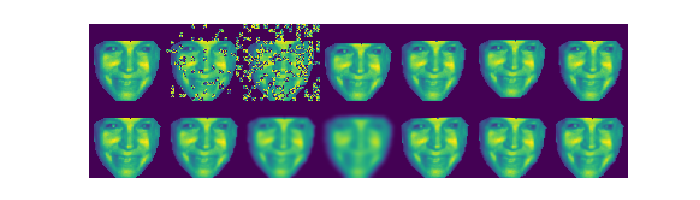
\includegraphics[scale=0.5]{augmenters}
        \end{figure}

    \subsection{Classifiers}
        \subsubsection{Convolutional Neural Network}
        We have used a convolutional neural network with the following structure:
        \begin{itemize}
            \item \textbf{Layers}:
            \begin{itemize}
            \item[$\blacksquare$] \textbf{conv. layer 0}: $20$ filters, $5 \text{x} 5$ kernel
            \item[$\blacksquare$] \textbf{max pooling}: $2 \text{x} 2$ pool size, $2 \text{x} 2$ strides
            \item[$\blacksquare$] \textbf{conv. layer 1}: $20$ filters, $5 \text{x} 5$ kernel
            \item[$\blacksquare$] \textbf{max pooling}: $2 \text{x} 2$ pool size, $2 \text{x} 2$ strides
            \item[$\blacksquare$] \textbf{conv. layer 2}: $40$ filters, $5 \text{x} 5$ kernel
            \item[$\blacksquare$] \textbf{max pooling}: $2 \text{x} 2$ pool size, $2 \text{x} 2$ strides
            \item[$\blacksquare$] \textbf{dense layer} with sigmoid activation function
            \end{itemize}
            \item \textbf{Loss function}: Log Loss
            \item \textbf{Optimizer}: SGD
            \item \textbf{Kernels initialization}: Since we have experimented with deeper
            networks too, and each model was trained from scratch, a reckless initialization
            would hamper the models ability to learn and increase the number of
            iterations needed for convergence. To ensure quick start of the learning
            process, we decided to initialize each kernel with \textbf{random normal
            distribution with $\mu = 0,\ \sigma = \sqrt{(2 / N)}$}, as advised by
            \citeauthor{initialization}.
        \end{itemize}


        \begin{figure}[H]
        \caption{Convolved input images (only IR channel). First two rows
        are outputs from first and second convolutional layers. Third and fourth
        row are outputs from all $40$ filters from last convolutional layer.
        }
        \centering
        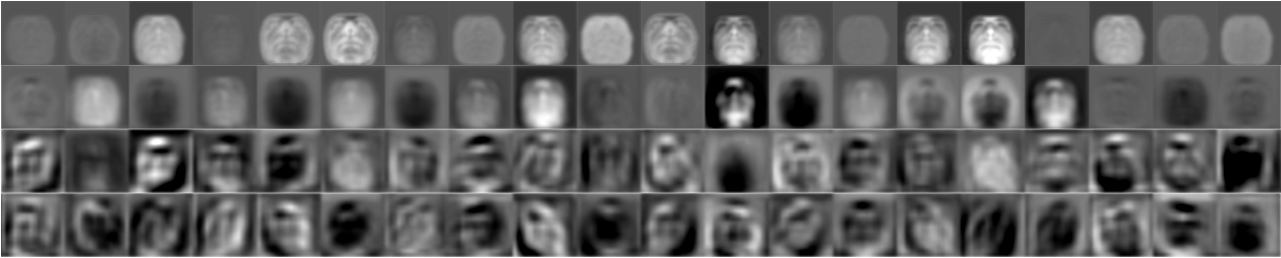
\includegraphics[scale=0.25]{convolutions}
        \end{figure}
        \begin{figure}[H]
            \caption{For each filter in each convolutional layer, $10$ patches
            among one of the test batches were chosen that activate those
            filters the most.
            Horizontally, consecutive filters are presented, vertically -- patches
            sorted from the highest activation.
            Note that from each patch, only IR channel is presented.
            }
            \centering
            \begin{subfigure}[b]{0.4\textwidth}
                \centering
                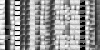
\includegraphics[scale=1.4]{exciting_layer0}
                \caption{conv. layer 0}
            \end{subfigure}
            \begin{subfigure}[b]{0.4\textwidth}
                \centering
                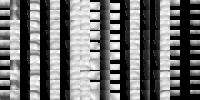
\includegraphics[scale=0.7]{exciting_layer1}
                \caption{conv. layer 1}
            \end{subfigure}
            \\
            \begin{subfigure}[b]{0.8\textwidth}
                \centering
                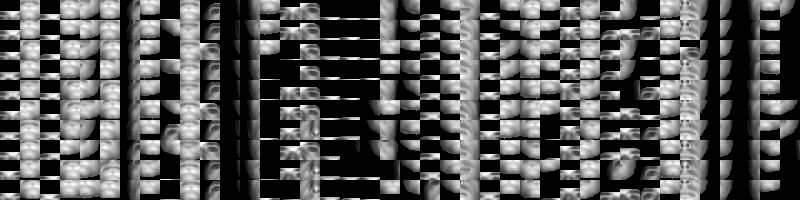
\includegraphics[scale=0.35]{exciting_layer2}
                \caption{conv. layer 2}
            \end{subfigure}
        \end{figure}

        \subsubsection{HOG + SVM}
        As an alterative to CNN, to classify HOG feature descriptors, we tested two common (\citeauthor{hog}, \citeauthor{rgbdhog}) approaches:
        Support Vector Machine, extremely randomised decision trees (Extra Trees), and both ensembled.
        Initially, while collecting the data and working with smaller dataset, Extra Trees where achieving higher results,
        and SVM was highly overfitting, but as the work proceeded, the second approach was getting better and has finally overcome Extra Trees
        to the point that the other classifier was not even contributing to ensembling, so further work was continued only with Support Vector Machines.
        In multi-class classification, we used One vs Rest approach.

        After tuning the parameters on final dataset using grid-search approach, the following configuration of most important parameters was chosen:
        \begin{itemize}
            \item \textbf{Polynomial kernel} with degree 3. Other kernels got significantly worse results.
            \item \textbf{Penalty C parameter}: 10, locally constant results results in range [1, 10].
            \item \textbf{Gamma parameter}: 0.7, locally constant results results in range [0.1, 1].
        \end{itemize}

        \subsubsection{Ensembling}
        We have experimented with a simple ensembling method -- voting.
        Each of our classifiers is implemented in a way that allows getting,
        apart from predictions, a vector of probabilities for each class.

        Let $C^{(1)}, C^{(2)}$ be two classifiers running in the same mode -- either
        binary or multi-class.
        Let $p_{C}(f)$ denote predicted probabilities for each class by classifier $C$,
        given input $f$.

        An ensembling classifier is configured by two values $w_1, w_2$ -- significance
        weights for classifiers $C^{(1)}, C^{(2)}$. Its output for input $f$ is defined as:
        \begin{center}
        $C_{E}(f) = \frac{w_{1} \cdot p_{C^{(1)}}(f) + w_{2} \cdot p_{C^{(2)}}(f)}{w_{1} + w_{2}}$
        \end{center}

        We will use notation $C^{(1)}\ w_{1}\ :\ w_{2}\ C^{(2)}$ to denote ensembling
        of classifiers $C^{(1)}$ and $C^{(2)}$ with weights $w_{1}, w_{2}$f.


    \subsection{Quality measures}
        Models have been trained in two modes: multi-class and binary
        classification. Let $T$ be the test set, $p_t$ -- predictions for test input
        $t \in T$ and $y_t$ -- ground truth for test input $t \in T$.
        \subsubsection*{Accuracy}
        For classifiers trained in multi-class mode the accuracy score has been
        measured:

        \begin{center}
        $acc(p, y) = \frac{|\{t \in T\ |\ p_t = y_t\}|}{|T|}$
        \end{center}

        \subsubsection*{Recall for fixed precision}

        When testing the model in binary mode two decisions are being made:
        \begin{itemize}
            \item \textbf{positive class (device owner)}: One subject from the
            database is chosen as the "device owner". All photos of this subjects
            are then labeled as positive. All photos of other subjects are
            labeled as negative.
            \item \textbf{desired precision threshold:}
            Precision is defined as:
            \begin{center}
            $prec(p, y) = \frac{\{t \in T\ |\ y_t = p_t = 1\}}{\{t \in T\ |\ p_t = 1\}}$
            \end{center}
            We have chosen $3$ different precision thresholds: $0.99$, $0.999$, $0.9999$.
        \end{itemize}
        Recall is defined as:
        \begin{center}
        $rec(p, y) = \frac{\{t \in T\ |\ p_t = y_t = 1\}}{\{t \in T\ |\ y_t = 1\}}$
        \end{center}
        For each precision threshold, we have calculated the corresponding recall measure and
        averaged the result over $5$ random choices for positive class.

    \begin{figure}[H]
    \caption{Test samples misclassified by CNN}
    \centering
    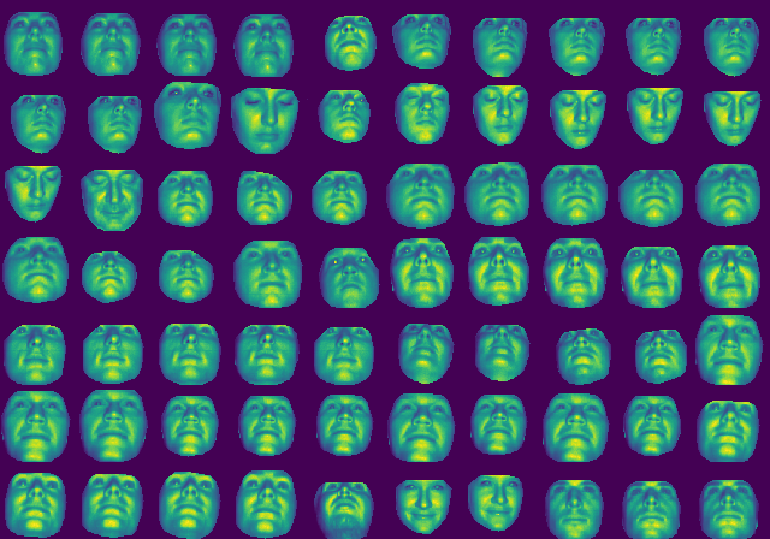
\includegraphics[scale=0.4]{misclassified}
    \end{figure}


    \subsection{Single-frame model results}
        We call a model single-frame if it classifies the person on the photo
        using only one frame. We have evaluated several single-frame models to
        choose one multi-class and one binary classifier.
        \subsubsection{Multi-class}
        \begin{table}[H]
        \begin{center}
        \small
        \caption{Selected models performance in multi-class mode}
        \begin{tabular}{ |c|c|c| }
            \hline
            Model & CNN inputs & Accuracy\\
            \hline
            CNN & channels & 0.9721\\
            \hline
            CNN 10 : 1 SVM + HOGs & channels & 0.9721\\
            \hline
            CNN 2 : 1 SVM + HOGs & channels & 0.9648\\
            \hline
            CNN 10 : 7 SVM + HOGs & channels & 0.9631\\
            \hline
            CNN 1 : 2 SVM + HOGs & channels & 0.9536\\
            \hline
            SVM + HOGs & - & 0.9099\\
            \hline
            CNN & concat & 0.8899\\
            \hline
        \end{tabular}
        \end{center}
        \end{table}

        \subsubsection{Binary}
        \begin{table}[H]
        \begin{center}
        \small
        \caption{Selected models performance in binary mode}
        \begin{tabular}{ |c|c|c|c| }
            \hline
            Model & CNN input & Precision & Recall\\
        \hline
        CNN 1 : 5 SVM + HOGs & channels & 0.99 & 0.9079\\
        & & 0.999 & 0.9013\\
        & & 0.9999 & 0.9013\\
        \hline
        SVM + HOGs & - & 0.99 & 0.8947 \\
        & & 0.999 & 0.8947\\
        & & 0.9999 & 0.8947\\
        \hline
        CNN & channels & 0.99 & 0.8487 \\
        & & 0.999 & 0.8487\\
        & & 0.9999 & 0.8487\\
        \hline
        CNN 1 : 1 SVM + HOGs & channels & 0.99 & 0.6908\\
        & & 0.999 & 0.6777\\
        & & 0.9999 & 0.6777\\
        \hline

        \end{tabular}
        \end{center}
        \end{table}

    \subsection{Multiple frames based classification}
    We have chosen CNN as multi-class classifier and CNN ensembled with SVM (CNN 1 : 5 SVM) as
    best performing single-frame classifiers.

    \subsubsection{Generating predictions from multiple frames}
    Let $n$ be the number of frames, $C_{1}$ -- a single-frame classifier and
    $f_1, ..., f_n$ be the $n$ consecutive frames.
    Let $p_{C_{1}}(f)$ denote the vector of probabilities predicted for each class by $C_{1}$,
    with frame $f$ as input.

    Note that $p_{C_{1}}(f) \in [0..1]^D$ where $D = 1$ for binary classification
    and $D$ equals to the number of classes in multi-class mode -- in our case $D = 44$.


    The multi-frame classifier $C_{n}$ can be defined as a function (namely arithmetic mean)
    from a tuple of $n$ frames to the vector of predicted probabilities:

    \begin{center}
    $C_{n}(f_1, ..., f_n) = \frac{\sum\limits_{i=1}^{n}{p_{C_{1}}(f_{i})}}{n}$
    \end{center}

    Another way of looking at multiple frames based classifier is as an ensembling
    of $n$ identical classifiers, but each receives a different frame as an input.

    \subsubsection{Frames-accuracy relation}
    \begin{figure}[H]
    \caption{Frames-accuracy relation for multiclass problem}
    \centering
    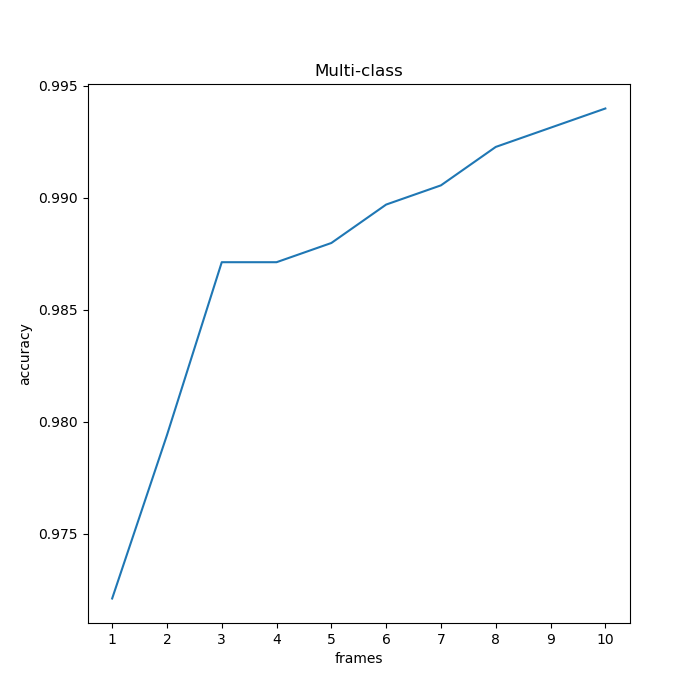
\includegraphics[scale=0.7]{multiclass_frames_accuracy_relation}
    \end{figure}

    \begin{figure}[H]
    \caption{Frames-accuracy relation for binary problem with precision threshold $\geqslant 0.99$}
    \centering
    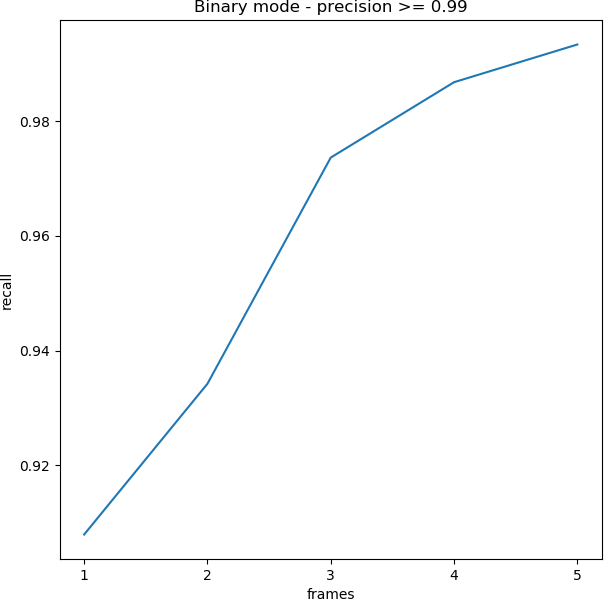
\includegraphics[scale=0.7]{binary_frames_recall_relation_099}
    \end{figure}

    \begin{figure}[H]
    \caption{Frames-accuracy relation for binary problem with precision threshold $\geqslant 0.999$}
    \centering
    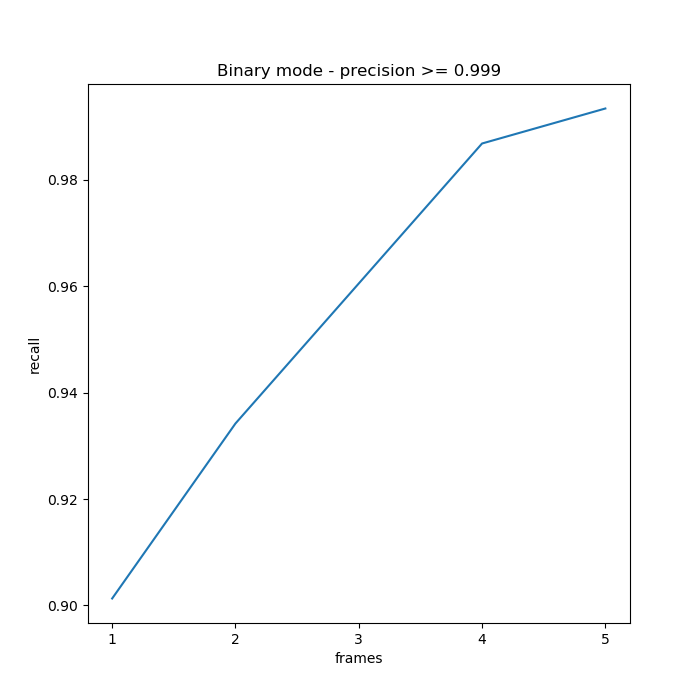
\includegraphics[scale=0.7]{binary_frames_recall_relation_0999}
    \end{figure}

    \begin{figure}[H]
    \caption{Frames-accuracy relation for binary problem with precision threshold $\geqslant 0.9999$}
    \centering
    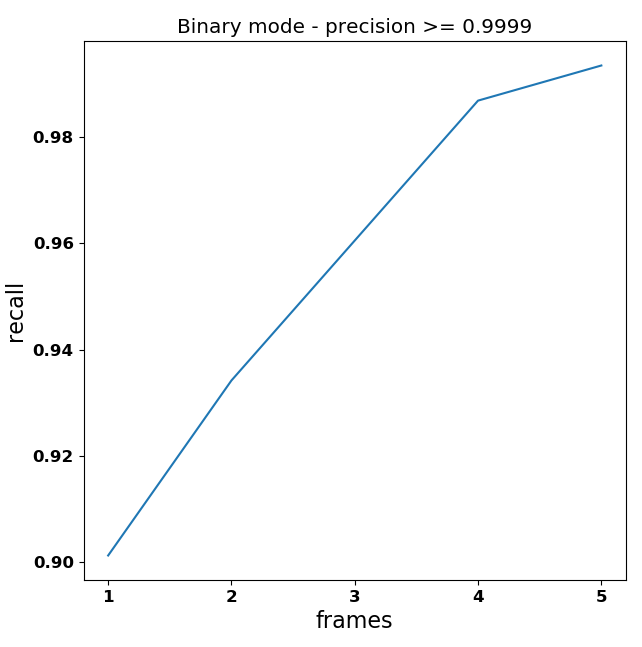
\includegraphics[scale=0.7]{binary_frames_recall_relation_09999}
    \end{figure}

    \subsubsection{Results -- multi-class}

    \begin{table}[H]
      \begin{center}
      \small
      \caption{Accuracy obtained by multi-frame based classification with CNN}
      \begin{tabular}{ |c|c| }
      \hline
      Frames & Accuracy\\
      \hline
      1 & 0.9721\\
      \hline
      2 & 0.9794\\
      \hline
      3 & 0.9871\\
      \hline
      4 & 0.9871\\
      \hline
      5 & 0.9879\\
      \hline
      6 & 0.9896\\
      \hline
      7 & 0.9905\\
      \hline
      8 & 0.9922\\
      \hline
      9 & 0.9931\\
      \hline
      10 & 0.9940\\
      \hline
      \end{tabular}
      \end{center}
    \end{table}

    \subsubsection{Results -- binary}
    \begin{table}[H]
    \begin{center}
    \small
    \caption{Recall obtained by multi-frame based classification with CNN 1 : 5 SVM}
    \begin{tabular}{ |c|c|c| }
        \hline
        Frames & Precision & Recall\\
    \hline
    1 & 0.99 & 0.9079\\
    & 0.999 & 0.9013\\
    & 0.9999 & 0.9013\\
    \hline
    2 & 0.99 & 0.9342\\
    & 0.999 & 0.9342\\
    & 0.9999 & 0.9342\\
    \hline
    3 & 0.99 & 0.9736\\
    & 0.999 & 0.9605\\
    & 0.9999 & 0.9605\\
    \hline
    4 & 0.99 & 0.9868\\
    & 0.999 & 0.9868\\
    & 0.9999 & 0.9868\\
    \hline
    5 & 0.99 & 0.9934\\
    & 0.999 & 0.9934\\
    & 0.9999 & 0.9934\\
    \hline

    \end{tabular}
    \end{center}
    \end{table}

    \subsection*{Possible improvements}

    \subsubsection*{Not tested approach to multi-frame classification}
    Instead of implementing multiple frame based classification as an ensembling
    of several single-frame classifiers, a single classifier could also be used.
    We believe that a recurrent neural network (RNN) might be a good fit for the
    task.

    \subsubsection*{Speed optimization}
    In our experiments, an external, heavy duty machine learning-based library
    has been used for finding and trimming faces (\ref{sec:trimming}). This has
    resulted in a single frame classification time of $260$ miliseconds -- most of
    which spent on detecting and trimming the face. This is too slow for $10$ FPS
    rate.

    We believe that a fully developed skin-recognition method, possibly with
    additional infrared channels on different wavelengths, could replace the
    all-in-one face detection library. Unfortunately, due to hardware limitations,
    we were unable to verify this assumption in our research.

    \subsection{Proposed solution}
    The solution we propose is a voting ensembling CNN 1 : 5 SVM, with
    classification based on $4$ consecutive frames. We believe that $400$ miliseconds
    is an acceptable authentication time. Using $4$ frames, precision rate $0.9999$
    and recall rate $0.9868$ are achievable.

    In other words, our solution will fail to protect users resources or device
    only once in $10\ 000$ cases. Out of $10\ 000$ cases when the right owner
    tries to access the device or resources, only $132$ times they will fail
    to authorize.

    \section{Conclusion}
    Face recognition based authentication methods have been around for a while. However,
    they have always been considered more of a gimmick rather than a serious
    authentication method. They are not secure enough and often are not reliable,
    for example because they don't work well in dark rooms.

    We believe our work shows that face recognition can become a secure and
    really trustworthy authentication method while being as or even more
    convenient than existing authentication methods.
    The tests on our database shows that the probability of accepting
    an unauthorized person is low enough to secure everything that is not top secret,
    and face recognition with a depth camera does not have most inconveniences
    of known bio-authentication methods -- such as fingerprint scanners not
    being usable in gloves or having to look directly at the camera for
    retina scanners.

    Additionally, we showed a proof of concept for skin recognition using
    hyperspectral images. We believe that with further research into
    using higher wavelengths or using more different wavelengths,
    which we were not able to do due to a lack of needed hardware,
    this could improve the security of face authentication even further.

    % We don't want to share this file, as
% there is nothing interesting inside...
% Just formal things for University.
% Sorry for inconvenience.

% \section{CD content}

% \section{How we were working?}

    \bibliography{bibliography}
\end{document}
